\documentclass[tikz]{standalone}
\usepackage{tikz}
\usetikzlibrary{positioning, graphs}
\usetikzlibrary{arrows.meta}
\usetikzlibrary{graphs.standard}
\begin{document}
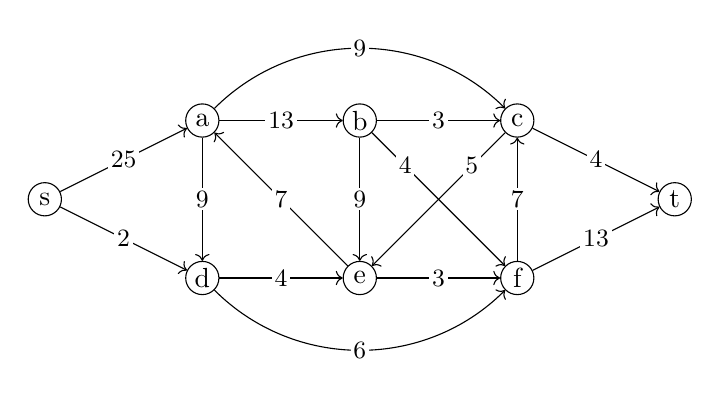
\begin{tikzpicture}
\begin{scope}
		[vertex/.style={draw,circle,inner sep = 0em, minimum size = 1.2em},
		 edgelabel/.style = {fill = white, inner sep = 0.1em, font=\small}]
		\node[vertex] (a) at (0,0) {a};
		\node[vertex] (b) at (2,0) {b};
		\node[vertex] (c) at (4,0) {c};
		\node[vertex] (d) at (0,-2) {d};
		\node[vertex] (e) at (2,-2) {e};
		\node[vertex] (f) at (4,-2) {f};
		\node[vertex] (s) at (-2,-1) {s};
		\node[vertex] (t) at (6,-1) {t};
		
		\draw[->] (s) to node[edgelabel] {$25$} (a);
		\draw[->] (s) to node[edgelabel] {$2$} (d);
		\draw[->] (a) to node[edgelabel] {$13$} (b);
		\draw[->, out=45, in = 135] (a) to node[edgelabel] {$9$} (c);
		\draw[->] (a) to node[edgelabel] {$9$} (d);
		\draw[->] (b) to node[edgelabel] {$3$} (c);
		\draw[->] (b) to node[edgelabel] {$9$} (e);
		\draw[->] (b) to node[edgelabel, near start] {$4$} (f);
		\draw[->] (c) to node[edgelabel] {$4$} (t);
		\draw[->] (c) to node[edgelabel, near start] {$5$} (e);
		\draw[->] (d) to node[edgelabel] {$4$} (e);
		\draw[->, out=-45, in=-135] (d) to node[edgelabel] {$6$} (f);
		\draw[->] (e) to node[edgelabel] {$7$} (a);
		\draw[->] (e) to node[edgelabel] {$3$} (f);
		\draw[->] (f) to node[edgelabel] {$7$} (c);
		\draw[->] (f) to node[edgelabel] {$13$} (t);
		
		
%		\draw[->] (s) to node[edgelabel] {$2$} (a);
%		\draw[->] (s) to node[edgelabel] {$8$} (e);
%		\draw[->] (s) to node[edgelabel] {$8$} (d);
%		\draw[->] (a) to node[edgelabel] {$7$} (e);
%		\draw[->] (a) to node[edgelabel, near start] {$7$} (f);
%		\draw[->] (b) to node[edgelabel] {$1$} (a);
%		\draw[->] (b) to node[edgelabel] {$1$} (c);
%		\draw[->] (c) to node[edgelabel] {$8$} (t);
%		\draw[->] (d) to node[edgelabel] {$5$} (e);
%		\draw[->, out = -45, in = -135] (d) to node[edgelabel] {$12$} (f);
%		\draw[->] (e) to node[edgelabel, near start] {$9$} (b);
%		\draw[->] (e) to node[edgelabel] {$5$} (f);
%		\draw[->] (f) to node[edgelabel] {$4$} (b);
%		\draw[->] (f) to node[edgelabel] {$4$} (c);
%		\draw[->] (f) to node[edgelabel] {$12$} (t);
		
\end{scope}
\end{tikzpicture}
\end{document}